\section{Deployment view}
\paragraph{}In this section we show how our components are really deployed on hardware devices.
\begin{figure}[H]
	\centering
	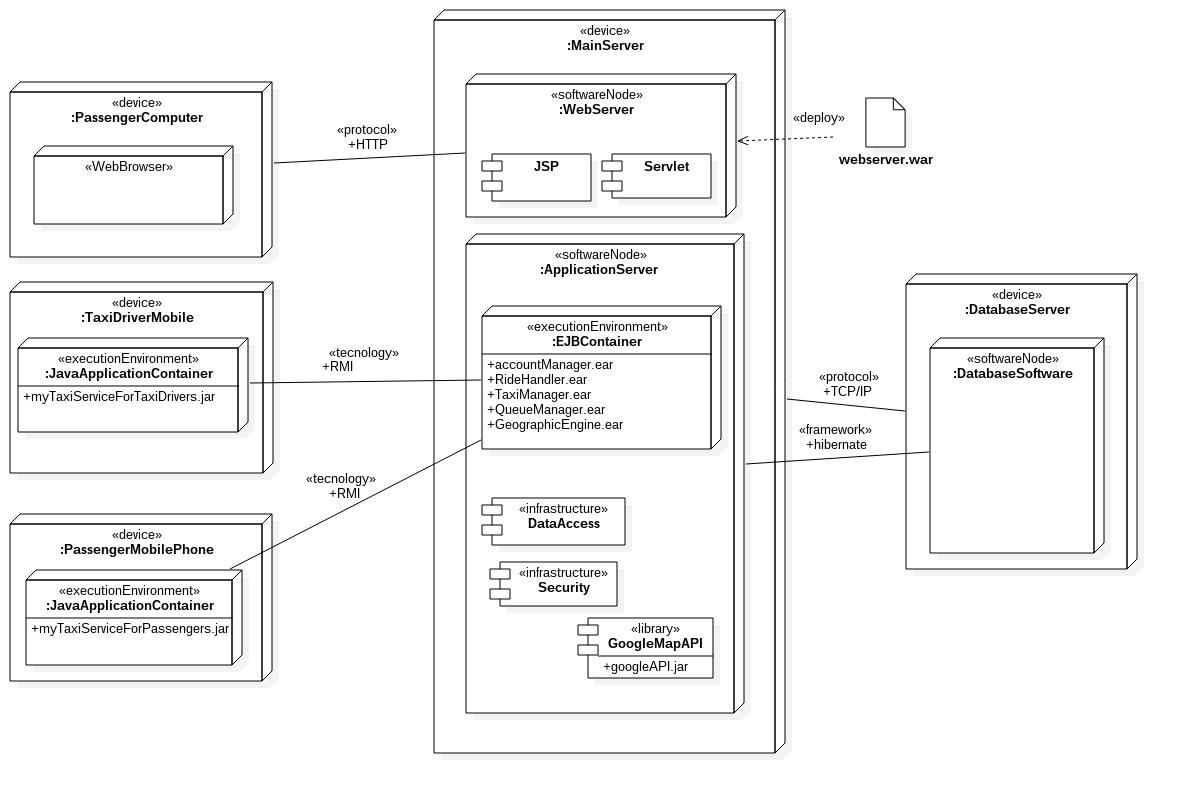
\includegraphics[trim=100 0 0 0,scale=0.35]{../"Analysis Documents"/deploymentView}
\end{figure}
\paragraph{} The UML diagram is self-explicative. We organize our deployed files like this:
\begin{itemize}
	\item \textit{Client side} we show the devices that can interact with our system: a mobile application and a browser for the passenger, and a mobile application for the taxi driver.
	\begin{itemize}
		\item The passenger and taxi driver client applications interact with the system through RMI calls
		\item The browser interact with the Web Server through HTTP protocol
	\end{itemize}
	\item \textit{Server side} both the web server and application server are deployed possibly in a cloud service, this will ensure the system to be reliable 24/24 7/7. The Application Server will keep all the components in a EJB pool so that it can handle the increased work load during specific time of the day, by deploying multiple instances of the stateless beans. It will also use the already specified infrastructural libraries for data access, security and the Google Maps API.
	\item The data are stored in multiple external \textit{databases} accessed by the Main Server through the Hibernate framework. There will be more than one instance of the database in order to make the whole system more reliable. Hibernate will abstract the fact that more than one database is been used, so the system is not aware of this.
\end{itemize}